%===========================================================
%                              Choix de track
%===========================================================
% Une des trois options 'parallelisme', 'architecture', 'systeme' 
% doit être utilisée avec le style compas2017
\documentclass[parallelisme]{compas2017}
\usepackage{comment}
\usepackage{graphicx}
\usepackage{listings}
\usepackage{tikz}
\usetikzlibrary{fit,positioning}

\pgfdeclarelayer{background}
\pgfsetlayers{background,main}

\newcommand\smalltt[1]{\texttt{\small #1}}

\graphicspath{{gfx/}}

\lstset{%
	basicstyle=\small\ttfamily,
	%frame=single
}

%===========================================================
%                               Title
%===========================================================

\toappear{1} % Conserver cette ligne pour la version finale

\begin{document}

\title{Méthode pour l'étude expérimentale par la simulation de clouds avec 
SCHIaaS.}
\shorttitle{SCHIaaS}

\author{Luke Bertot, Julien Gossa, Stéphane Genaud}% A voir l'ordre. 
% - Stéphane: moi en dernier.

\address{Université De Strasbourg,\\
Laboratoire ICube - Pôle API - 300 Bd Sébastien Brant\\
67400 Illkirch-Graffenstaden - France\\
lbertot@unistra.fr gossa@unistra.fr genaud@unistra.fr }

\date{\today}

\maketitle

%===========================================================         %
%R\'esum\'e
%===========================================================  
\begin{abstract}

Les clouds ont été intensivement étudiés les dernières années, que ce soit du 
point de vue de l'administrateur qui doit par exemple décider de l'emplacement
des machines virtuelles sur l'infrastructure matérielle, ou du client qui doit 
décider du dimensionnement de sa plateforme virtuelle. Pour ce faire, de 
nombreux
simulateurs ont vu le jour. Malheureusement, ces derniers se limitent souvent à 
mimer les fonctionnalités d'un cloud. Ils manquent d'ancrage dans la 
réalité, en raison d'une part d'une absence de comparaison à des exécutions réelles, 
et d'autre part d'un ensemble de traces réelles injectables dans les 
simulations. De plus, ils ne proposent pas un cadre complet d'étude
des résultats obtenus, pourtant indispensable à la reproductibilité des 
expériences et la comparaison de solutions différentes.
Le projet SCHIaaS vise à combler ces deux manques. Cet article ce focalise sur 
ce dernier point, en présentant un \textit{framework} d'étude par la 
simulation de bout-en-bout, de la conception du simulateur à l'analyse des 
résultats.

  \MotsCles{simulation ; cloud ; reproductibilité }
\end{abstract}


%=========================================================
\section{Introduction}
%=========================================================

Les  clouds  sont  devenus  ces  dernières  années  une  brique  essentielle  de
l'informatique,   omni-présents  dans   les   architectures   de  nos   systèmes
d'information. La compréhension de leurs  comportements est donc un enjeu majeur
qui a incité les chercheurs à proposer des simulateurs de cloud, essentiellement
pour les clouds de type \textit{Infrastructure-as-a-Service} (IaaS). Ces
simulateurs   reposent   sur   une   modélisation  que l'on peut qualifier de
\textit{bottom-up} : les ressources matérielles sont d'abord modélisées, puis le
comportement des  machines virtuelles sur  ces ressources matérielles,  puis les
applications s'exécutant dans cet environnement. On peut donc distinguer dans 
de nombreux outils de simulation trois composants : 
\begin{itemize}
		\item une spécification de plateforme
		\item une spécification de l'application.
		\item un modèle de simulation
\end{itemize}

Le modèle de simulation forme le cœur d'un simulateur. Il décrit l'évolution de
l'état de tous  les composants du système  simulé en fonction du  temps et des
évènements.   Il  repose  sur  des   modèles  individuels  pour  chacun  de  ces
composants  (réseau,  processeur,  \ldots).   Etant  donné  la  complexité  du
comportement   des   composants,  les   modèles   actuels   procèdent  à   des
simplifications, ce qui engendre des écarts avec la réalité. La précision des 
modèles utilisés est le principal élément discriminant
entre simulateurs, l'utilisateur  n'ayant généralement que peu de  prise sur cet
aspect%
\footnote{SimGrid  permet  néanmoins  de  choisir  différents  modèles  pour  le
  réseau}.

La spécification de plateforme décrit  l'environnement simulé.  Elle est fournie
par l'utilisateur et décrit les caractéristiques techniques de l'infrastructure,
comme la topologie  d'interconnexion, la puissance des  processeurs, la capacité
des liens réseaux,  etc.  Le niveau de détail de  cette description, qui diffère
selon les simulateurs, influence également la précision de la simulation.

La  spécification   de  l'application,   fournie  par  l'utilisateur,   est  une
description de la  séquence des évènements à simuler.  Les simulateurs existants
privilégient cette  description sous la forme  d'un programme qui, à  l'aide des
primitives  de  la  bibliothèque  de  simulation,  décrit  le  comportement  des
opération  réelles simulées.   Mais d'autres  mode de  description peuvent  être
proposés,   comme   l'injection  d'une   trace   d'exécution   réelle,  ou   une
représentation abstraite de suite d'opérations. 

Le tableau suivant
donne un aperçu des possibilités des principaux simulateurs du domaine, en 
terme d'application : (a) trace d'exécution, (b) représentation abstraite, (c) 
simulation  programmée ; de performance CPU : (d) délai mesuré, (e) délai
utilisateur ; de réseau : (flow) analytique ou (packet) niveau paquet ; et 
enfin de disque.

\begin{center}
\begin{tabular}{|c||c|c|c||c|c|c|c|}
	\hline
	%% line 1
	& \multicolumn{3}{c|}{Application} &
	\multicolumn{2}{c|}{CPU}&Réseau&Disque\\
	\cline{2-8}
	%%line 2
	Simulator &(a) 
                  &(b)
                  &(c)
                  &(d)
                  &(e)&
	type & precision max\\
	\hline
	%%line 3
	CloudSim\cite{cloudsim} & & & \bf X &&\bf
	X&store\&forward&seek+transfert\\ \hline
	ICanCloud\cite{icancloud} & & & \bf X &&\bf X&packet& bloc \\ \hline
	GroudSim\cite{groudsim} & & & \bf X &&\bf X&flot& n/a\\\hline
	GreenCloud\cite{greencloud} & & \bf X &&&\bf X&packet& n/a\\ \hline
	SimGrid\cite{simgrid}& \bf X & \bf X & \bf X &\bf X&\bf X& flot/packet &
	seek+transfert \\
	\hline
\end{tabular}
\end{center}

Une fois le simulateur réalisé, l'expérimentateur peut étudier le 
comportement de ses composants en observant les traces de ses exécutions, 
parfois en très grand nombre. Les observations arrivent donc seulement en fin 
de processus. Or, l'étude de ces observations mènent souvent à des 
modifications du simulateur, ainsi que du choix des observations pertinentes. Il 
faudrait ensuite refaire toutes les simulations et toutes les observations, ce 
qui est une tâche fastidieuse souvent négligée par l'expérimentateur qui se 
limite aux quelques simulations et observations qui lui paraissent pertinentes 
sur l'instant. Ce processus artisanal est source d'erreur dans la compréhension 
des phénomènes simulés : n'appliquant pas les mêmes observations à toutes les 
simulations, certaines choses peuvent échapper à l'expérimentateur.

L'objet  de cet  article est  de  présenter le  \textit{framework} SCHIaaS,  qui
repose sur  SimGrid, et  qui grâce  à un  outil appelé  \emph{le lab}  permet de
standardiser  les  études  par  simulation  afin  d'éviter  ces  travers.   Nous
présentons  d'abord ce  \textit{framework} dans  la section~\ref{sec:framework},
puis  un cas  d'utilisation concret  en section~\ref{sec:usecase}  et enfin  une
conclusion en section~\ref{sec:conclusion}.




%=========================================================
\section{Présentation du \textit{framework}} \label{sec:framework}
%=========================================================


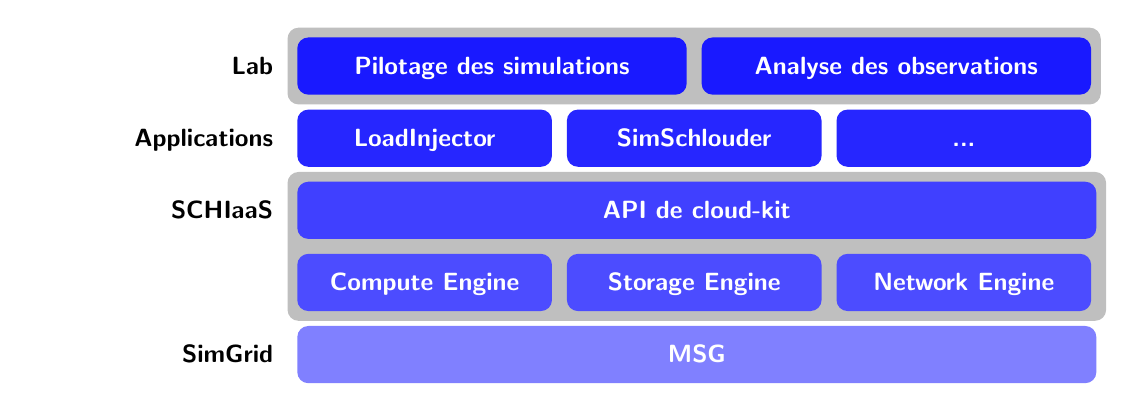
\begin{tikzpicture}[node distance=5pt,
level/.style={
  font={\sffamily\bfseries\color{black} \fontsize{9pt}{12}\selectfont},
  align=right,
  text width=3cm,
  text height=10pt,
  text depth=4pt},
module1/.style={
  level,
  font={\sffamily\bfseries\color{white} \fontsize{9pt}{12}\selectfont},
  rounded corners,
  text width=9cm+26pt,
  align=center},
module2/.style={
  module1,
  text width=4.5cm+6pt},
module3/.style={
  module1,
  text width=3cm},
moduleset/.style={
  rounded corners,
  fill=lightgray},
]

\node[level] (Lab) {Lab};
\node[module2,right=of Lab,fill=blue!90] (labpy) {Pilotage des 
simulations};
\node[module2,right=of labpy,fill=blue!90] (TU) {Analyse des 
observations};
\begin{pgfonlayer}{background}
\node[moduleset, fit=(labpy) (TU)] {};
\end{pgfonlayer}

\node[level,below=of Lab] (App) {Applications};
\node[module3,right=of App,fill=blue!85] (LI) {LoadInjector};
\node[module3,right=of LI,fill=blue!85] (SS) {SimSchlouder};
\node[module3,right=of SS,fill=blue!85] () {...};

\node[level,below=of App] (SCHIaaS) {SCHIaaS};
\node[module1,right=of SCHIaaS,fill=blue!75] (API) 
{API de \textit{cloud-kit}};
\node[level,below=of SCHIaaS] (SCHIaaS2) {};
\node[module3,right=of SCHIaaS2,fill=blue!70] (CE) {Compute Engine};
\node[module3,right=of CE,fill=blue!70] (SE) {Storage Engine};
\node[module3,right=of SE,fill=blue!70] (NE) {Network Engine};
\begin{pgfonlayer}{background}
\node[moduleset, fit=(API) (CE) (SE) (NE)] {};
\end{pgfonlayer}

\node[level,below=of SCHIaaS2] (SG) {SimGrid};
\node[module1,right=of SG,fill=blue!50] (SG) {MSG};



\end{tikzpicture}


\subsection{SCHIaaS et SimGrid}


SimGrid~\cite{simgrid}  est un  simulateur à  évènements discrets  qui permet  à
l'utilisateur d'exprimer la modélisation  d'une application distribuée à travers
un  programme utilisant  des  primitives  qui  décrivent  les phases  de
communications et de calcul des différents processus applicatifs. Ces primitives
sont disponibles à travers différentes interfaces, adaptées aux systèmes étudiés
; il  existe par exemple  des interface  pour les applications  pair-à-pair, MPI
(SMPI), les workflows sous forme de DAG (SimDAG), ou les processus communicants
de type CSP (MSG).

Le  travail présenté  dans  cet article  repose sur  une  nouvelle interface  de
SimGrid,  nommée SCHIaaS pour \textit{Simulation of Cloud, Hypervisor and 
IaaS}.  Nous  ne
présentons ici que quelques éléments saillants de SCHIaaS mais le lecteur pourra
trouver  une  description  détaillée  sur  le  site  dédié~\cite{schiaas-gforge}.
SCHIaaS  est  un  \textit{framework}   permettant  le  développement  rapide  de
simulateurs de cloud. Il peut être utilisé pour évaluer des algorithmes au 
niveau du gestionnaire de cloud (appelée aussi \textit{cloud-kit},  par exemple
OpenStack), mais aussi au niveau d'applications clientes d'un cloud.

Développé en JAVA, il offre un ensemble de classes prédéfinies représentant tous
les composants d'un cloud kit. L'utilisateur qui souhaite insérer sa description
du  comportement d'un  ou plusieurs  composants, peut  rapidement greffer  cette
description sous la forme d'un programme  qui vient spécialiser l'une ou l'autre
de ces classes.


% ----- inutile maintenant -----
% Le tout  est facilement  instrumentable par  un ensemble  de scripts,
%appelé \emph{lab},  qui permet d'automatiser l'exécution  des simulations, leurs
%observations, et l'analyse des résultats.

La simulation du fonctionnement du  niveau \textit{cloud-kit} est assuré par des
moteurs, exposant les fonctionnalités des clouds au niveau administrateur :
\begin{itemize}
 \item Compute : moteur d'instanciation et de gestion des VM;
 \item Storage : moteur de gestion des stockages;
 \item Network : moteur de gestion de la virtualisation du réseau.
\end{itemize}

Chacun de  ces moteurs est  une interface abstraite  assurant l'interopérabilité
entre  eux  ainsi  qu'avec  les   autres  niveaux  du  \textit{framework}.   Des
implémentations de ces  moteurs sont fournies, permettant  d'avoir un simulateur
par défaut pleinement fonctionnel.   Ces implémentations imitent le comportement
d'OpenStack. Un développeur  de fonctionnalités administrateur n'a  donc qu'à se
concentrer sur  la partie  qui l'intéresse, par  exemple différents  systèmes de
stockages.

Les ordonnanceurs de machines virtuelles (VM), qui décident sur quelles machines
physiques  (PM)  seront  déployées  les  VM  demandées  par  l'utilisateur,  ont
également  leur interface  abstraite.  Plusieurs ordonnanceurs  par défaut  sont
fournis,  sur l'exemple  d'Openstack  qui  permet au  choix  d'équilibrer ou  de
consolider les charges  des machines physiques au moyen d'un  poids calculé pour
chacune d'elles.

Un  système abstrait  d'injection de  charge  est également  fourni. Ce  dernier
permet de  contrôler un  nombre de  VM déployées et  les charges  de ces  VM, en
particulier  CPU.   

Ces interfaces ne sont  que celles utilisées dans la suite  de l'article à titre
d'illustration, mais tous les composant d'un \textit{cloud-kit} sont présents
dans SCHIaaS.  
% --- repetition -----
%Chaque module peut être remplacé, étendu, ou
%utilisé en l'état,  ce qui permet le prototypage rapide  de simulateurs de cloud
%adaptés à l'étude de l'utilisateur, sans qu'il  ait à développer plus que ce qui
%l'intéresse.

\subsection{Applications}

SCHIaaS ne peut s'exécuter seul. Dans  la philosophie SimGrid, un simulateur est
une  application exploitant  les fonctionnalités  fournies, mais  qui doit  être
développée et  compilée.  Cette philosophie  est conservée avec SCHIaaS,  qui ne
fait qu'étendre les  fonctionnalités de SimGrid avec celles  disponibles dans un
cloud.

Cependant, deux applications sont fournies par défaut: 
\begin{itemize}
\item \emph{LoadInjector}, qui permet d'injecter  une charge utilisateur sans se
  préoccuper des  applications qui s'exécutent  dans les  VM. Il est  utile pour
  mener des études au niveau administrateur.
  Deux injecteurs  par défaut  sont  fournis. Le  premier est  un  simple 
injecteur  de charges sinusoïdales  entièrement paramétrables.  Le second 
injecte  les charges observées  sur  l'infrastructure  de  Google,   et  rendue 
 disponible  en tant que google cluster-data\cite{gcd}.
\item  \emph{SimSchlouder},  qui   est  la  version  simulée   du  système  réel
  Schlouder\cite{Michon2017}.  Il s'agit d'un  courtier de ressources virtuelles
  capable   de  piloter   de   concert   un  ordonnanceur   de   tâches  et   un
  \textit{cloud-kit}  pour  exécuter  des   calculs  scientifiques  sur  clouds.
\end{itemize}

\subsection{Le Lab}

Le lab est un ensemble de scripts permettant d'automatiser l'exécution des simulations, la collecte des
observations, ainsi que leur analyse. Il permet donc d'exécuter de bout-en-bout l'étude par simulation,
de la définition des différentes simulations, à la production des graphiques.

Au delà de l'aspect pratique et du gain de temps de mise en œuvre de l'étude, le lab a pour vocation
de ``standardiser'' l'étude. Cette standardisation assure sa reproductibilité, ainsi qu'une comparaison
équitable entre solutions à un même problème.

Mais le lab permet également une approche systématique permettant à 
l'expérimentateur de ne pas rater de phénomène. En effet, il est fréquent de 
faire un grand lot de simulations, plus d'observer plus finement celles qui 
présentent des particularités. Ce faisant, l'expérimentateur exclu les autres 
simulation de ces observations plus précises, à moins de les refaire 
entièrement. En rendant plus pratique la définition des observations 
directement au niveau du \textit{workflow} de simulations, le lab assure que 
tous les cas seront observés de la même manière, ce qui évite de rater un 
phénomène, ou de différencier le traitement des simulations au risque d'arriver 
à des conclusions abusives.


\section{Cas d'usage concret} \label{sec:usecase}

Plaçons nous dans le cas du problème, parfois appelé \textit{VM Packing}, de 
l'ordonnancement des VMs sur les machines physiques. 
Supposons que l'on dispose d'un algorithme visant à reconsolider 
régulièrement les VMs, c'est à dire à les concentrer sur le moins de PMs 
possibles en les migrant, et que l'on souhaite étudier l'impact du \emph{délai}
entre ces reconsolidations sur le \emph{nombre de PMs utilisées} et sur le 
\emph{nombre de migrations} nécessaires, lorsque le cloud est soumis à une 
charge sinusoïdale.

Pour mener cette étude, les différentes étapes sont :
\begin{enumerate}
 \itemsep0em
 \item la conception du simulateur ;
 \item la description du contexte expérimental des simulations ;
 \item la description et l'exécution des simulations ;
 \item l'analyse des résultats.
\end{enumerate}


\subsection{Conception du simulateur}

Notre \textit{framework} permet de partir sur la base d'un simulateur pleinement 
fonctionnel en sélectionnant les modules par défaut pertinents pour l'étude. 
Les développements se limitent alors strictement aux parties spécifiques à 
l'étude.

Dans le contexte de cette étude, le développement concernera seulement 
l'interface \smalltt{ComputeScheduler}, qu'il faudra implanter avec l'algorithme 
étudié. Des implantations génériques fournies par défaut facilitent ce 
développement. En l'occurrence, il suffira de spécialiser 
\smalltt{SimpleReconfigurator}, qui reconfigure le placement des VMs avec un 
\emph{délai} configurable.

Tous les autres modules sont ceux par défaut, et ne nécessitent même pas d'être 
maîtrisés.

Le problème étudié est purement administrateur, seule compte la charge en terme 
de nombre de VMs et de CPU de ces VMs, peu importe les applications qui y sont 
exécutées. Nous allons donc utiliser l'application \emph{LoadInjector}, dont la 
fonction principale est \smalltt{loadinjector.SimpleInjection} et qui charge 
simplement un injecteur dans la simulation.

\subsection{Description du contexte expérimental des simulations}

La description du contexte expérimental des simulations se fait au travers de 
fichiers xml, respectant le format standard de SimGrid :

\begin{description}
	\item[platform.xml] décrit l'infrastructure matérielle : machines 
physiques et réseau.
	\item[deploy.xml] décrit les processus.
	\item[cloud.xml] décrit la plateforme de cloud : hôtes,
types d'instance, et ordonnanceurs.
	\item[injector.xml] décrit les injecteurs à utiliser.
\end{description}

Dans notre cas, \smalltt{deploy.xml} est inutile, mais il faudra produire 
\smalltt{platform.xml} et \smalltt{cloud.xml}, ou utiliser les exemples fournis.

Nous allons comparer les résultats avec des délais de reconsolidation de $0$, 
$10$ et $100$. Il faudra donc décliner le fichier de configuration du cloud 
pour ces trois cas : \smalltt{cloud-reconsolidator0.xml}, 
\smalltt{cloud-reconsolidator10.xml} et \smalltt{cloud-reconsolidator100.xml}. 

De plus, il faudra configurer l'injecteur, par exemple en utilisant 
\smalltt{SinInjector} qui injecte une charge de calcul sinusoïdale sur un nombre 
de VMs suivant également une sinusoïde.


\subsection{Description et exécution des simulations}

L'exécution d'une simulation se fait avec la commande suivante : 
\begin{lstlisting}
$ java  loadinjector.SimpleInjection platform.xml deploy.xml cloud.xml
injector.xml
\end{lstlisting}

Toutes les expérience du \emph{lab} sont guidées par un fichier de 
configuration. Celui ci contient l'ensemble des informations nécessaires aux 
simulations, les variables à observer, et si nécessaire les pré- ou post- 
traitements requis. 

Les lignes \smalltt{TU\_ARG} permettent de définir les observations que nous 
souhaitons faire, en l'occurrence le nombre de machines dont le nombre de cœurs 
utilisés n'est pas nul, ainsi que le nombre de VM en état de migration.

Les lignes \smalltt{SIM\_ARG} donnent les arguments des simulations à faire. 
En l'occurrence, le quatrième argument doit prendre successivement les trois 
fichiers de configuration correspondants au trois ordonnanceurs à comparer. 
Le lab exécute toutes les combinaisons d'arguments possibles, ainsi il est 
facile de démultiplier les simulations. Par exemple, l'ajout d'une ligne 
\smalltt{SIM\_ARG 5} permettrait de faire les mêmes simulations, mais avec 
deux injecteurs différents.

La commande \smalltt{./lab.py -p 4 cmp-scheduler.cfg} permet d'exécuter 
notre expérience, avec 4 simulations en parallèle, grâce au fichier :

\begin{lstlisting}
# setup
SETUP_DIR ./setup/cmp-scheduler
NEEDED_POST template.R
POST_COMMAND_DATA R -f template.R > R.out

# observations
TU_ARG --count-if used_cores ne 0
TU_ARG --count-if vm:.*:state eq migrating

# simulations
SIM_ARG 1 loadinjector.SimpleInjection
SIM_ARG 2 platform.xml 
SIM_ARG 3 deploy.xml
SIM_ARG 4:reconsolidator0 cloud-reconsolidator10.xml
SIM_ARG 4:reconsolidator10 cloud-reconsolidator10.xml 
SIM_ARG 4:reconsolidator100 cloud-reconsolidator100.xml
SIM_ARG 5 injector.xml
\end{lstlisting}


\subsubsection{Analyse des résultats}

A la fin des exécution le \emph{lab} extrait des traces de simulation les 
observations demandées et les stocke dans des fichiers séparés, puis exécute 
les commandes stipulées par les lignes \smalltt{$POST\_COMMAND$}. En 
l'occurrence, il s'agit d'un patron R, utilisant une librairie inclue dans le 
lab :

\begin{lstlisting}
pdf('data.pdf')
dfs <- tu_read('.', plotting=TRUE, plotting_state=FALSE)
dev.off()
\end{lstlisting}

Ce dernier va automatiquement produire un graphique pour chaque observation 
demandée, comme montré Figure \ref{output}.

\begin{figure}[]
	
	\caption{Graphiques produits automatiquement par le lab.}
	\begin{tabular}{ccc}
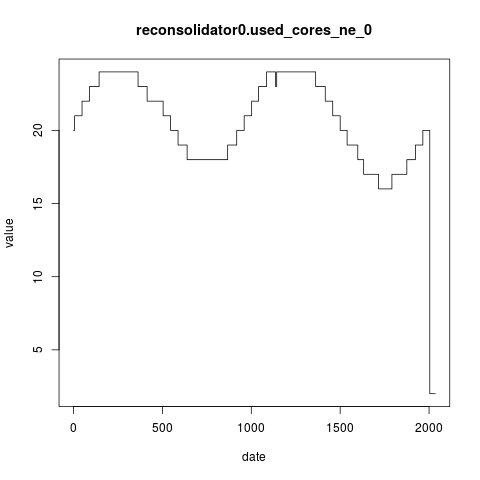
\includegraphics[scale=0.30]{reconsolidator0_used_cores_ne_0}&
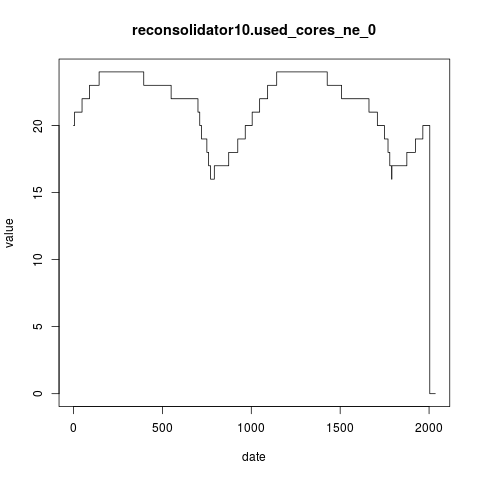
\includegraphics[scale=0.30]{reconsolidator10_used_cores_ne_0}&
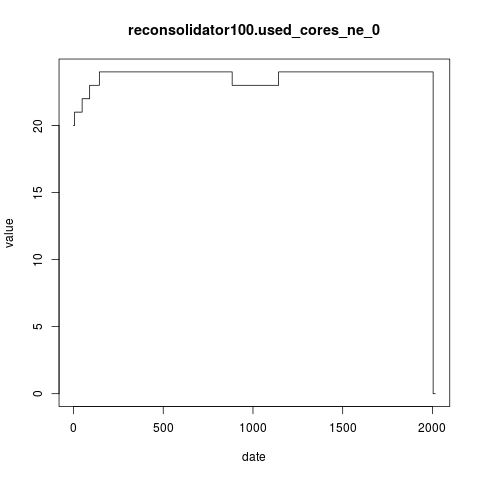
\includegraphics[scale=0.30]{reconsolidator100_used_cores_ne_0}\\
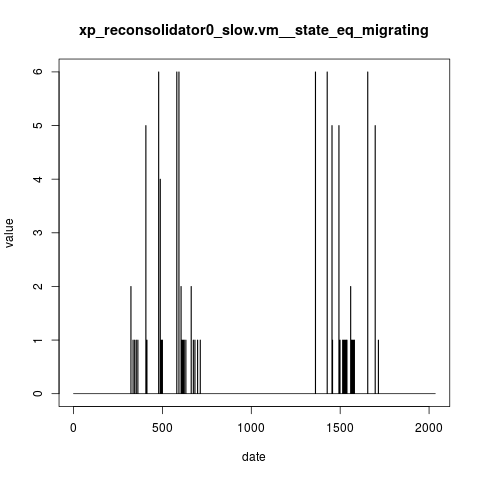
\includegraphics[scale=0.30]{xp_reconsolidator0_slow_vm__state_eq_migrating}&
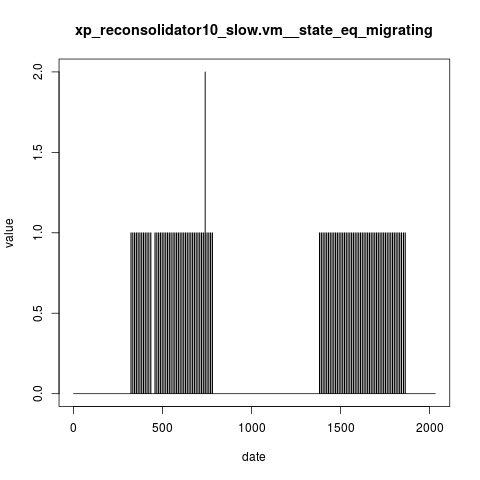
\includegraphics[scale=0.30]{xp_reconsolidator10_slow_vm__state_eq_migrating}&
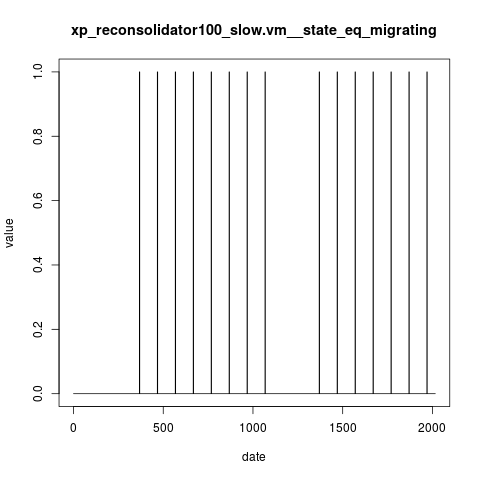
\includegraphics[scale=0.30]{xp_reconsolidator100_slow_vm__state_eq_migrating}\\
	\end{tabular}
	\label{output}
\end{figure}

On peut observer  sur ces six graphiques qu'un intervalle de reconsolidation nul
permet d'optimiser le  nombre de machines utilisées, mais au  prix de nombreuses
migrations concurrentes (quantité sur l'axe \textit{value}), qu'un intervalle de
100  secondes ne  présente aucun  intérêt  en terme  d'optimisation, mais  qu'un
intervalle  de 10  secondes optimise  raisonnablement la  plateforme, en  évitant
quasiment toute migration  concurrente.  Il est important de remarquer également
que  ces   graphiques ont les travers inévitables
des   données  produites automatiquement : titres abscons, labels   génériques,
et   échelles  par défaut. L'utilisateur souhaitant raffiner ces données devra
adapter le fichier \texttt{template.R}.

%=========================================================
\section{Conclusion} \label{sec:conclusion}
%=========================================================

Le  \emph{lab}  est un  outil  pour  l'automatisation d'exécution  d'expériences
\emph{in  silico} qui  permet  d'exécuter facilement  de multiples  simulations.
L'automatisation  des simulation  et des  observations permet  non seulement  de
s'assurer que rien  n'échappe à l'expérimentateur, mais  rend aussi l'expérience
trivialement reproductible.   Le \emph{lab} est  déjà utilisé au seins  de notre
équipes pour  la validation de  SCHIaaS, en simulant  automatiquement l'ensemble
d'une   archive  de   273  exécutions   réelles,  chacune   dans  5   conditions
expérimentales  différentes, soit  plus de  1300 simulations  à observer.   Nous
l'utilisons également  pour des simulations de  Monte Carlo, en procédant  à des
lots de  500 simulations  afin d'approcher  l'évaluation des  performances d'une
application  dont les  temps d'exécution  sont difficilement  modélisables.  Des
études par la  simulation de tels volumes sont pratiquement  impossibles à mener
sans  un outil  support à  la méthodologie  de l'expérimentation  permettant une
étude de bout-en-bout.




\bibliography{biblio}

\end{document}



\subsection{SimSchlouder}

L'application \emph{SimSchlouder} permet le prototypage rapide de simulateurs pour évaluer les 
algorithmes d'ordonnancement de VM et de tâches au niveau utilisateurs du cloud. 
Dans ces cas là, l'état de l'infrastructure interne du cloud importe peu, seule compte le service 
rendu à l'utilisateur, isolé sur sa propre plateforme virtuelle. 

Schlouder\cite{Michon2017} est un courtier de ressources virtuelles. Il prend en
entrée la description d'une charge de travail, au format slurm citation???
étendu de quelques informations permettant d'adapter le courtage aux besoins
utilisateurs. Ensuite, Schlouder analyse la charge de travail soumise, et 
décide
à l'aide d'algorithmes de dimensionnement (\textit{provisioning}) de déployer un
certains nombres de VM, puis ordonnance les tâches sur ces VMs, et étend les VMs
lorsqu'elles sont devenues inutiles.

SimSchlouder est l'alter-égo de Schlouder, dont l'architecture, les fonctionnalités, le comportement
et les entrées/sorties sont entièrement reproduite dans SCHIaaS. La description d'une charge de 
travail peut donc être soumise indifféremment à Schlouder pour une exécution 
réelle, ou à SimSchlouder
pour une évaluation des choix de courtage par la simulation. Une option de Schlouder permet 
d'ailleurs d'appeler directement SimSchlouder, et d'obtenir le temps de 
complétion et le prix 
de l'exécution demandée en fonction de la plateforme de cloud cible et de la stratégie de réservation
de VM choisie.

Les stratégies d'évaluation des réservations de ressources de cloud ont été intensivement étudiées 
ces dernières années. Cependant, elles sont rarement comparées entre elles, et leur évaluation 
est souvent basée sur des simulations ad-hoc ou inadaptées, et des charges de travail purement artificielles.
SimSchlouder permet de rapidement développer de telles stratégies, et de comparer leurs performances 
à celles fournies par défaut, à savoir ASAP (\textit{As Soon As Possible}, qui vise à minimiser le temps de 
complétion) et AFAP (\textit{As Full As Possible}, qui vise à minimiser les réservations de ressources,
et donc le coût). De plus, cette comparaison peut s'appuyer sur les traces récupérées lors de l'utilisation 
de l'application réelle Schlouder. Pour l'instant, nous mettons à disposition 481 traces d'exécutions
sur deux plateformes : notre cloud privé, homogène, stable et non partagé, et BonFire qui est un cloud 
public hétérogène, instable et partagé, dont les différents sites ont des comportements et des matériels 
assez différents pour qu'on les considère ocmme des clouds différents.
Les charges de travail sont issues de deux applications : OMSSA, qui est un sac de tâches assez courtes 
en protéomique, et MONTAGE, qui est un \textit{workflow} en astronomie ayant des tâches plus imposantes. 

Ainsi, l'utilisation de SimSchlouder permet de ne développer que le c\oe{}ur 
d'un stratégie de réservation 
de ressources, simplement en implémentant une interface abstraite très simple, 
pour pouvoir comparer cette 
stratégie aux autres dans des contextes applicatifs et matériels nombreux, représentatifs, et réellement 
éprouvés.

Ces comparaisons nécessitent de très nombreuses simulations, c'est pourquoi nous avons conçu \emph{le lab}.




\begin{enumerate}
	\item Mise en place
		\begin{description}
			\item[SETUP\_DIR] dossier où se trouve tout les fichiers
			\item[POST\_COMMAND\_DATA] commande a exécuter sur les
				observations
			\item[NEEDED\_POST] fichiers requit par 
POST\_COMMAND\_DATA 
		\end{description}
		Il est possible d'exécuter des commandes avant simulation
		(PRE\_COMMAND\_SETUP), ou d'injecter d'autre fichier de commande
		(INCLUDE) eventuelement eux même écrit par la précommande.
	\item Simulations
		\begin{description}
			\item[SIM\_ARG $n$:nom] ensemble des arguments à
				passer au simulateur indexé par leur position
				$n$. Le \emph{lab} exécutera une simulation
				pour chaque combinaison d'arguments possible.
				Pour que index ou plusieurs argument sont
				possible un nom et requit pour différencié les
				simulations.
		\end{description}
		Les l'ensemble des fichiers écrit par chaque simulation sont 
placé
		dans un dossier nommé d'après les argument de la simulation.
	\item Observation
		\begin{description}
			\item[TU\_ARG] ensemble de filtre a appliquer au traces
				de simulation.
		\end{description}
		Les fichier obtenu grâce a TU\_ARGS permettent d'observer les
		variables pertinente de la simulation sans avoir a fouiller
		l'ensemble des traces verbeuses de SCHIaaS. Cette étape est
		cruciale pour l'exploitation automatique des résultats
\end{enumerate}
